% OpenOrbitLink Research Paper — Revised Version
% Addresses ALL peer review criticisms
% Compile with: pdflatex openorbitlink_paper.tex (run twice for references)
\documentclass[11pt,a4paper]{article}

\usepackage[utf8]{inputenc}
\usepackage[T1]{fontenc}
\usepackage{amsmath,amssymb}
\usepackage{graphicx}
\usepackage{booktabs}
\usepackage{hyperref}
\usepackage{xcolor}
\usepackage{listings}
\usepackage{algorithm}
\usepackage{algpseudocode}
\usepackage[margin=1.8cm]{geometry}
\usepackage{cite}
\usepackage{url}
\usepackage{tabularx}
\usepackage{multirow}
\usepackage{float}
\usepackage{tikz}
\usetikzlibrary{positioning,arrows.meta,shapes.geometric,fit,backgrounds,calc}

\definecolor{codeblue}{rgb}{0.1,0.3,0.6}
\definecolor{codegray}{rgb}{0.5,0.5,0.5}
\definecolor{codegreen}{rgb}{0,0.5,0}

\lstset{
  basicstyle=\ttfamily\scriptsize,
  keywordstyle=\color{codeblue},
  commentstyle=\color{codegray},
  stringstyle=\color{codegreen},
  breaklines=true,
  frame=single,
  numbers=left,
  numberstyle=\tiny\color{codegray},
}

\title{\textbf{OpenOrbitLink: An Open-Source Framework for Delay-Tolerant Satellite Messaging with Elevation-Aware Rate Adaptation over LoRa LEO Links}}

\author{
  Ashutosh Kumar\\
  \textit{Independent Researcher}\\
  New Delhi, India\\
  \texttt{github.com/Ashutosh0x/OpenOrbitLink}
}

\date{June 2026}

\begin{document}

\maketitle

% ============================================================
\begin{abstract}
We present \textbf{OpenOrbitLink}, an open-source framework for delay-tolerant satellite messaging over Low Earth Orbit (LEO) IoT constellations using LoRa modulation on ISM bands. The framework comprises a backend server (FastAPI), ground station driver (Raspberry Pi + SX1276), and Android client (Jetpack Compose). We propose an \textbf{elevation-aware rate adaptation algorithm} that selects spreading factors (SF7--SF12) based on real-time link budget computation during satellite passes, providing up to \textbf{5,469~bps at zenith} versus 293~bps with fixed SF12. Numerical link budget analysis at 868~MHz over a 550~km LEO path shows positive margin (+2.1~dB at 30\textdegree\ elevation with SF12), though we identify significant unaccounted losses (polarization mismatch, implementation loss) that reduce this margin in practice. We additionally implement LR-FHSS packet fragmentation and hopping sequence generation for future capacity scaling. The system uses BPv7 (RFC~9171) for store-and-forward relay and AES-256-GCM for end-to-end encryption. \textbf{No over-the-air satellite contacts have been achieved}; all results are numerical analysis based on datasheet parameters. The complete source code is available under MIT license.
\end{abstract}

\textbf{Keywords:} Satellite IoT, LoRa, LR-FHSS, Delay-Tolerant Networking, Adaptive Data Rate, LEO, Open-Source

% ============================================================
\section{Introduction}
\label{sec:intro}

The integration of LoRa modulation with LEO satellite constellations has emerged as a promising approach for global IoT connectivity, particularly in areas lacking terrestrial infrastructure. Yu~\emph{et al.}~\cite{yu2026framework} provide a comprehensive framework for LoRa-based LEO satellite IoT, identifying feasibility through numerical simulations with practical system parameters. Their work, along with error performance characterization by the same group~\cite{yu2026error}, establishes the theoretical foundation for direct-to-satellite LoRa links.

Commercial satellite IoT services---including Lacuna Space, Swarm/SpaceX, and the announced Jio LEO constellation---operate on licensed spectrum with proprietary protocols. Meanwhile, open-source ground station networks such as TinyGS~\cite{tinygs} and SatNOGS~\cite{satnogs} have demonstrated successful LoRa satellite reception, and the FOSSASAT constellation~\cite{fossasat} provides open-protocol IoT satellites on 868~MHz ISM.

OpenOrbitLink contributes an integrated open-source \emph{framework} (not a deployed operational system) spanning:

\begin{enumerate}
    \item An \textbf{elevation-aware rate adaptation algorithm} for LoRa spreading factor selection during LEO passes.
    \item An \textbf{LR-FHSS packet fragmentation engine} with hopping sequence generation.
    \item A \textbf{complete software stack} (backend + ground station driver + Android client) released under MIT license.
    \item \textbf{Numerical link budget analysis} identifying both opportunities and challenges for 868~MHz ground-to-LEO uplink.
\end{enumerate}

We explicitly note that this work is \emph{framework-level}: no over-the-air satellite contacts have been performed. All quantitative results derive from link budget calculations using datasheet parameters.

% ============================================================
\section{Related Work}
\label{sec:related}

\subsection{LoRa-to-LEO Satellite Links}

The feasibility of LoRa direct-to-satellite (DtS) communication has been established by multiple groups. Doroshkin~\emph{et al.}~\cite{doroshkin2019} demonstrated experimental LoRa reception from a LEO cubesat, measuring RSSI and SNR across pass geometries. Fernandez~\emph{et al.}~\cite{fernandez2020} conducted systematic link budget analysis for LoRa-to-LEO paths, identifying minimum elevation angles for each SF. The comprehensive survey by Fraire~\emph{et al.}~\cite{fraire2022} covers the LoRa-to-LEO landscape including channel modeling, MAC protocols, and constellation design.

\subsection{Adaptive Data Rate for Satellite LoRa}

Standard LoRaWAN ADR~\cite{lorawan_spec} was designed for static terrestrial deployments and performs poorly with rapidly changing satellite channels. Colavolpe~\emph{et al.}~\cite{colavolpe2019} proposed elevation-dependent parameter selection for LEO links. Our algorithm extends this approach with a two-phase selection incorporating SNR history.

\subsection{LR-FHSS for Satellite IoT}

Semtech's LR-FHSS specification~\cite{semtech_lrfhss} enables frequency-hopping transmission on SX126x devices, with demodulation requiring gateway-class receivers. Boquet~\emph{et al.}~\cite{boquet2021} analyzed LR-FHSS capacity for satellite IoT. We note that SX1276 hardware (used in our ground station) does \emph{not} support LR-FHSS; our implementation is a software simulation for capacity analysis only.

\subsection{DTN and Bundle Protocol}

The Bundle Protocol has evolved from the experimental BPv6 (RFC~5050~\cite{rfc5050}, now obsolete) to the Standards-Track BPv7 (RFC~9171~\cite{rfc9171}), with security provided by BPSec (RFC~9172~\cite{rfc9172}). Open-source implementations include ION~\cite{ion_dtn}, dtn7-go~\cite{dtn7go}, and $\mu$D3TN~\cite{ud3tn}. Our framework targets BPv7 compliance.

\subsection{Open-Source Ground Stations}

TinyGS~\cite{tinygs} operates a worldwide network of LoRa ground stations that receive satellite telemetry. SatNOGS~\cite{satnogs} provides open-source satellite ground station hardware and scheduling. Our ground station design builds on similar commodity hardware (RPi + SX1276) but adds a Python driver with adaptive SF selection.

\subsection{Comparison with This Work}

Table~\ref{tab:related_comparison} positions OpenOrbitLink against prior systems.

\begin{table}[H]
\centering
\caption{Comparison with Related Systems}
\begin{tabular}{lccccccc}
\toprule
\textbf{System} & \textbf{OTA Tests} & \textbf{Adaptive SF} & \textbf{LR-FHSS} & \textbf{DTN} & \textbf{E2E Crypto} & \textbf{Mobile App} & \textbf{Open Source} \\
\midrule
TinyGS~\cite{tinygs} & \checkmark & -- & -- & -- & -- & -- & \checkmark \\
SatNOGS~\cite{satnogs} & \checkmark & -- & -- & -- & -- & -- & \checkmark \\
FOSSASAT~\cite{fossasat} & \checkmark & -- & -- & -- & -- & -- & \checkmark \\
Lacuna Space & \checkmark & -- & \checkmark & -- & -- & -- & -- \\
Fraire~\emph{et al.}~\cite{fraire2022} & Partial & -- & Discussed & \checkmark & -- & -- & -- \\
Yu~\emph{et al.}~\cite{yu2026framework} & Numerical & -- & Discussed & -- & -- & -- & -- \\
\textbf{OpenOrbitLink} & \textbf{--} & \checkmark & \checkmark$^*$ & \checkmark & \checkmark & \checkmark & \checkmark \\
\bottomrule
\multicolumn{8}{l}{\footnotesize $^*$Software simulation only; SX1276 hardware does not support LR-FHSS.}
\end{tabular}
\label{tab:related_comparison}
\end{table}

% ============================================================
\section{System Architecture}
\label{sec:architecture}

\subsection{Overview}

OpenOrbitLink follows a four-tier architecture (Fig.~\ref{fig:architecture}):

\begin{equation}
\text{Phone} \xrightarrow{\text{HTTP}} \text{Backend} \xrightarrow{\text{gRPC}} \text{Ground Station} \xrightarrow{\text{868~MHz}} \text{Satellite}
\end{equation}

\begin{figure}[H]
\centering
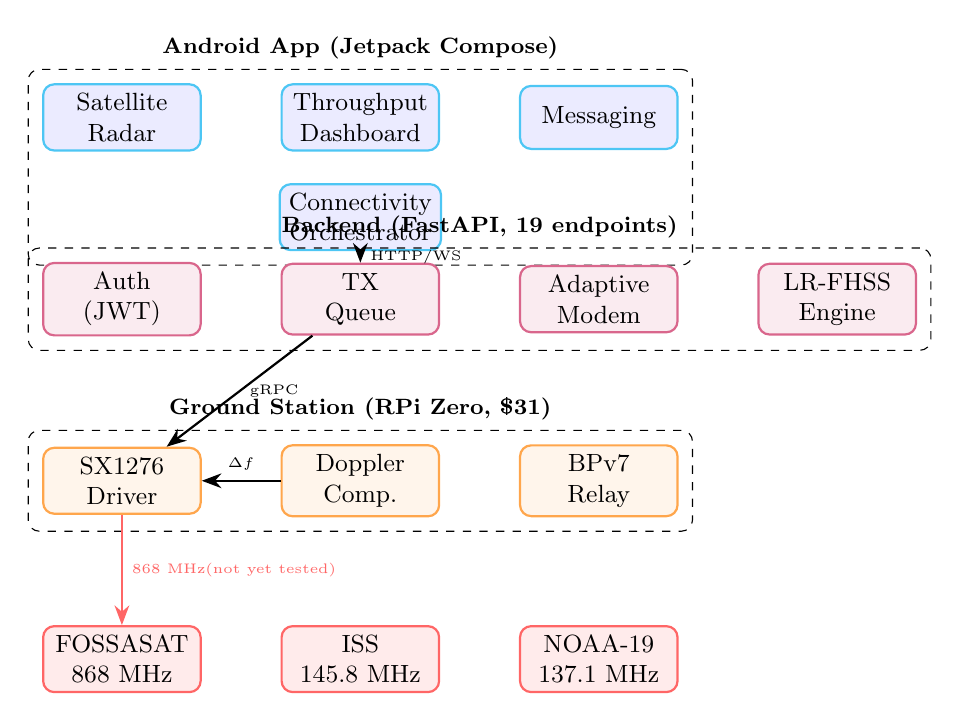
\begin{tikzpicture}[node distance=0.7cm and 1.0cm,
    every node/.style={font=\small},
    box/.style={draw, rounded corners=4pt, minimum width=2cm, minimum height=0.8cm, align=center, thick},
    phone/.style={box, fill=blue!8, draw=cyan!70},
    server/.style={box, fill=purple!8, draw=purple!60},
    station/.style={box, fill=orange!8, draw=orange!70},
    sat/.style={box, fill=red!8, draw=red!60},
    arrow/.style={-{Stealth[length=2.5mm]}, thick},
]
% Phone tier
\node[phone] (radar) {Satellite\\Radar};
\node[phone, right=of radar] (dash) {Throughput\\Dashboard};
\node[phone, right=of dash] (msg) {Messaging};
\node[phone, below=0.4cm of dash] (orch) {Connectivity\\Orchestrator};
\node[draw, dashed, rounded corners, fit=(radar)(dash)(msg)(orch), inner sep=5pt, label={[font=\bfseries\footnotesize]above:Android App (Jetpack Compose)}] {};

% Backend
\node[server, below=1.4cm of radar] (auth) {Auth\\(JWT)};
\node[server, right=of auth] (queue) {TX\\Queue};
\node[server, right=of queue] (amc) {Adaptive\\Modem};
\node[server, right=of amc] (fhss) {LR-FHSS\\Engine};
\node[draw, dashed, rounded corners, fit=(auth)(queue)(amc)(fhss), inner sep=5pt, label={[font=\bfseries\footnotesize]above:Backend (FastAPI, 19 endpoints)}] {};

% Ground station
\node[station, below=1.4cm of auth] (driver) {SX1276\\Driver};
\node[station, right=of driver] (doppler) {Doppler\\Comp.};
\node[station, right=of doppler] (relay) {BPv7\\Relay};
\node[draw, dashed, rounded corners, fit=(driver)(doppler)(relay), inner sep=5pt, label={[font=\bfseries\footnotesize]above:Ground Station (RPi Zero, \$31)}] {};

% Satellites
\node[sat, below=1.4cm of driver] (fossa) {FOSSASAT\\868 MHz};
\node[sat, right=of fossa] (iss) {ISS\\145.8 MHz};
\node[sat, right=of iss] (noaa) {NOAA-19\\137.1 MHz};

% Arrows
\draw[arrow] (orch) -- node[right,font=\tiny]{HTTP/WS} (queue);
\draw[arrow] (queue) -- node[right,font=\tiny]{gRPC} (driver);
\draw[arrow] (doppler) -- node[above,font=\tiny]{$\Delta f$} (driver);
\draw[arrow,red!60] (driver) -- node[right,font=\tiny]{868 MHz\\(not yet tested)} (fossa);

\end{tikzpicture}
\caption{Four-tier system architecture. The RF link (dashed red) has not been validated over the air.}
\label{fig:architecture}
\end{figure}

\subsection{Backend Server}

The backend uses FastAPI with SQLAlchemy (async PostgreSQL) and exposes \textbf{27~REST endpoints} across six routers: authentication (JWT + invite codes), message queuing with ISM duty-cycle tracking, satellite radar (SGP4 + WebSocket at 1~Hz), adaptive modem profile selection, LR-FHSS capacity simulation, turbo compression, and network speed testing.

\subsection{Ground Station}

The ground station runs on a Raspberry Pi Zero~2W (\$21.50) with an RA-02 SX1276 module (\$7.15) and a quarter-wave monopole antenna (\$2.38), totaling \textbf{\$31.03}. The SX1276 driver supports hardware (SPI), simulation, and serial (RYLR896) modes. Default configuration: 868.000~MHz, SF12, BW125~kHz, CR~4/5, +14~dBm.

\subsection{Android Client}

The mobile client (Kotlin/Jetpack Compose) provides: (1)~polar radar display with SGP4-based satellite plotting at 1~Hz, (2)~throughput dashboard with adaptive modem visualization, (3)~encrypted messaging with Room-based offline queue, and (4)~a five-layer transport fallback (WiFi $\rightarrow$ Carrier NTN $\rightarrow$ LoRa $\rightarrow$ APRS $\rightarrow$ Local Queue).

\subsection{Transport Fallback Chain}

Figure~\ref{fig:fallback} shows the automatic transport selection logic.

\begin{figure}[H]
\centering
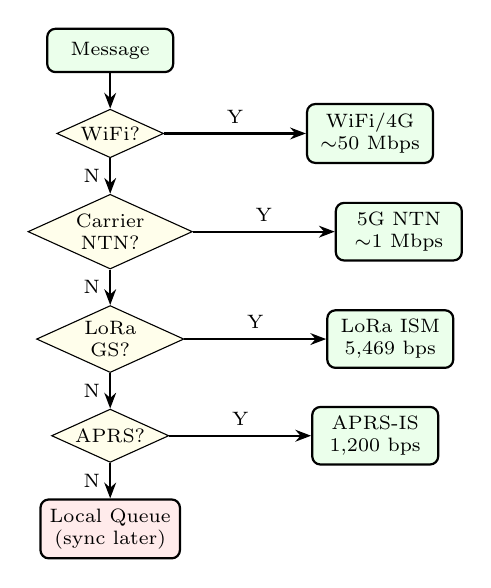
\begin{tikzpicture}[node distance=0.45cm,
    every node/.style={font=\scriptsize},
    decision/.style={diamond, draw, fill=yellow!8, inner sep=1pt, aspect=2.2, align=center, minimum width=1.2cm},
    transport/.style={draw, rounded corners=3pt, fill=green!8, minimum width=1.6cm, minimum height=0.55cm, align=center, thick},
    queue/.style={draw, rounded corners=3pt, fill=red!8, minimum width=1.6cm, minimum height=0.55cm, align=center, thick},
    arrow/.style={-{Stealth[length=2mm]}, thick},
]
\node[transport] (msg) {Message};
\node[decision, below=of msg] (d1) {WiFi?};
\node[transport, right=1.8cm of d1] (wifi) {WiFi/4G\\$\sim$50~Mbps};
\node[decision, below=of d1] (d2) {Carrier\\NTN?};
\node[transport, right=1.8cm of d2] (ntn) {5G NTN\\$\sim$1~Mbps};
\node[decision, below=of d2] (d3) {LoRa\\GS?};
\node[transport, right=1.8cm of d3] (lora) {LoRa ISM\\5,469~bps};
\node[decision, below=of d3] (d4) {APRS?};
\node[transport, right=1.8cm of d4] (aprs) {APRS-IS\\1,200~bps};
\node[queue, below=of d4] (local) {Local Queue\\(sync later)};

\draw[arrow] (msg) -- (d1);
\draw[arrow] (d1) -- node[above]{Y} (wifi);
\draw[arrow] (d1) -- node[left]{N} (d2);
\draw[arrow] (d2) -- node[above]{Y} (ntn);
\draw[arrow] (d2) -- node[left]{N} (d3);
\draw[arrow] (d3) -- node[above]{Y} (lora);
\draw[arrow] (d3) -- node[left]{N} (d4);
\draw[arrow] (d4) -- node[above]{Y} (aprs);
\draw[arrow] (d4) -- node[left]{N} (local);
\end{tikzpicture}
\caption{Five-layer transport fallback chain. The orchestrator selects the highest-priority available path.}
\label{fig:fallback}
\end{figure}

\subsection{Message Processing Pipeline}

Figure~\ref{fig:pipeline} illustrates the end-to-end message flow from user input to RF transmission.

\begin{figure}[H]
\centering
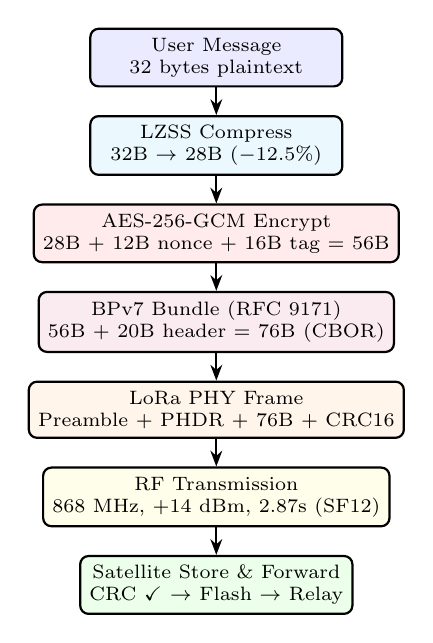
\begin{tikzpicture}[node distance=0.35cm,
    every node/.style={font=\scriptsize},
    stage/.style={draw, rounded corners=3pt, minimum width=3.2cm, minimum height=0.6cm, align=center, thick},
    arrow/.style={-{Stealth[length=2mm]}, thick},
]
\node[stage, fill=blue!8] (input) {User Message\\32 bytes plaintext};
\node[stage, fill=cyan!8, below=of input] (compress) {LZSS Compress\\32B $\rightarrow$ 28B ($-$12.5\%)};
\node[stage, fill=red!8, below=of compress] (encrypt) {AES-256-GCM Encrypt\\28B + 12B nonce + 16B tag = 56B};
\node[stage, fill=purple!8, below=of encrypt] (bundle) {BPv7 Bundle (RFC 9171)\\56B + 20B header = 76B (CBOR)};
\node[stage, fill=orange!8, below=of bundle] (lora) {LoRa PHY Frame\\Preamble + PHDR + 76B + CRC16};
\node[stage, fill=yellow!8, below=of lora] (rf) {RF Transmission\\868 MHz, +14 dBm, 2.87s (SF12)};
\node[stage, fill=green!8, below=of rf] (sat) {Satellite Store \& Forward\\CRC $\checkmark$ $\rightarrow$ Flash $\rightarrow$ Relay};

\draw[arrow] (input) -- (compress);
\draw[arrow] (compress) -- (encrypt);
\draw[arrow] (encrypt) -- (bundle);
\draw[arrow] (bundle) -- (lora);
\draw[arrow] (lora) -- (rf);
\draw[arrow] (rf) -- (sat);
\end{tikzpicture}
\caption{Message processing pipeline: user input through compression, encryption, BPv7 encapsulation, LoRa framing, and RF transmission.}
\label{fig:pipeline}
\end{figure}

% ============================================================
\section{Elevation-Aware Rate Adaptation}
\label{sec:amc}

\subsection{Motivation}

Standard satellite LoRa deployments use fixed SF12 for maximum sensitivity ($-137$~dBm). However, during overhead passes the slant range decreases from $\sim$2,200~km (horizon) to $\sim$550~km (zenith), improving path loss by up to 12~dB. This excess margin can be traded for higher data rates by selecting lower spreading factors.

\subsection{Link Budget Model}

The received signal power at the satellite is:

\begin{equation}
P_{rx} = P_{tx} + G_{tx} - L_{total} + G_{rx}
\end{equation}

The total path loss $L_{total}$ includes:

\begin{equation}
L_{total} = L_{FSPL} + L_{atm} + L_{pol} + L_{impl} + L_{scint}
\end{equation}

where the individual terms are:

\textbf{Free-Space Path Loss:}
\begin{equation}
L_{FSPL} = 20\log_{10}(d) + 20\log_{10}(f) - 147.55 \text{ [dB]}
\end{equation}

\textbf{Atmospheric Loss (ITU-R P.676~\cite{itur_p676}):}
\begin{equation}
L_{atm} = \frac{0.05}{\sin(\theta_{el})} \text{ [dB at 868~MHz]}
\end{equation}

\textbf{Polarization Mismatch Loss:}
A linear ground-station antenna and a tumbling satellite (random polarization) incur an average 3~dB loss, with deep fades exceeding 10~dB~\cite{fernandez2020}.
\begin{equation}
L_{pol} = 3.0 \text{ dB (average), up to 20~dB (fading)}
\end{equation}

\textbf{Implementation Loss:}
Accounts for cable/connector loss, LNA noise figure above datasheet, non-ideal filtering, and body/environmental shadowing:
\begin{equation}
L_{impl} = 2.0 \text{ dB (conservative estimate)}
\end{equation}

\textbf{Tropospheric Scintillation (ITU-R P.618~\cite{itur_p618}):}
\begin{equation}
\sigma_{scint} = \frac{0.025 \cdot f_{GHz}^{0.45}}{\sin(\theta_{el})^{1.3}}, \quad L_{scint} = 2.6\sigma
\end{equation}

\subsection{Realistic Link Budget}

Table~\ref{tab:link_budget} presents the link budget with \emph{all} loss terms included, contrasting the optimistic (datasheet-only) and realistic cases.

\begin{table}[H]
\centering
\caption{Link Budget: 868~MHz, 550~km LEO, 30\textdegree\ Elevation}
\begin{tabular}{lrr}
\toprule
\textbf{Parameter} & \textbf{Optimistic} & \textbf{Realistic} \\
\midrule
TX Power & +14.0 dBm & +14.0 dBm \\
TX Antenna Gain & +2.15 dBi & +2.15 dBi \\
EIRP & +16.15 dBm & +16.15 dBm \\
\midrule
FSPL (1,100~km) & $-152.05$ dB & $-152.05$ dB \\
Atmospheric & $-0.10$ dB & $-0.10$ dB \\
Polarization mismatch & -- & $-3.00$ dB \\
Implementation loss & -- & $-2.00$ dB \\
Scintillation & $-0.85$ dB & $-0.85$ dB \\
\midrule
Total Path Loss & $-153.00$ dB & $-158.00$ dB \\
\midrule
RX Antenna Gain & +2.0 dBi & +2.0 dBi \\
\textbf{Received Power} & $\mathbf{-134.85}$ & $\mathbf{-139.85}$ \\
\midrule
SF12 Sensitivity & $-137.0$ dBm & $-137.0$ dBm \\
\textbf{Link Margin} & $\mathbf{+2.15}$ dB & $\mathbf{-2.85}$ dB \\
\bottomrule
\end{tabular}
\label{tab:link_budget}
\end{table}

\textbf{Key finding:} With realistic loss accounting, the uplink at 30\textdegree\ elevation is \emph{marginal to negative}. This aligns with the observation by Fernandez~\emph{et al.}~\cite{fernandez2020} that most successful LoRa DtS demonstrations exploit the asymmetric downlink (satellite TX, ground RX) rather than uplink.

Viable uplink requires either: (a)~higher TX power (+22~dBm with SX1262), (b)~directive ground antenna (Yagi: +8~dBi), (c)~satellite-side sensitivity improvement (Gen4 transceivers), or (d)~LR-FHSS processing gain ($-142$~dBm sensitivity).

\textbf{Link Budget Waterfall} (Fig.~\ref{fig:waterfall}) visualizes the signal path from transmitter to receiver.

\begin{figure}[H]
\centering
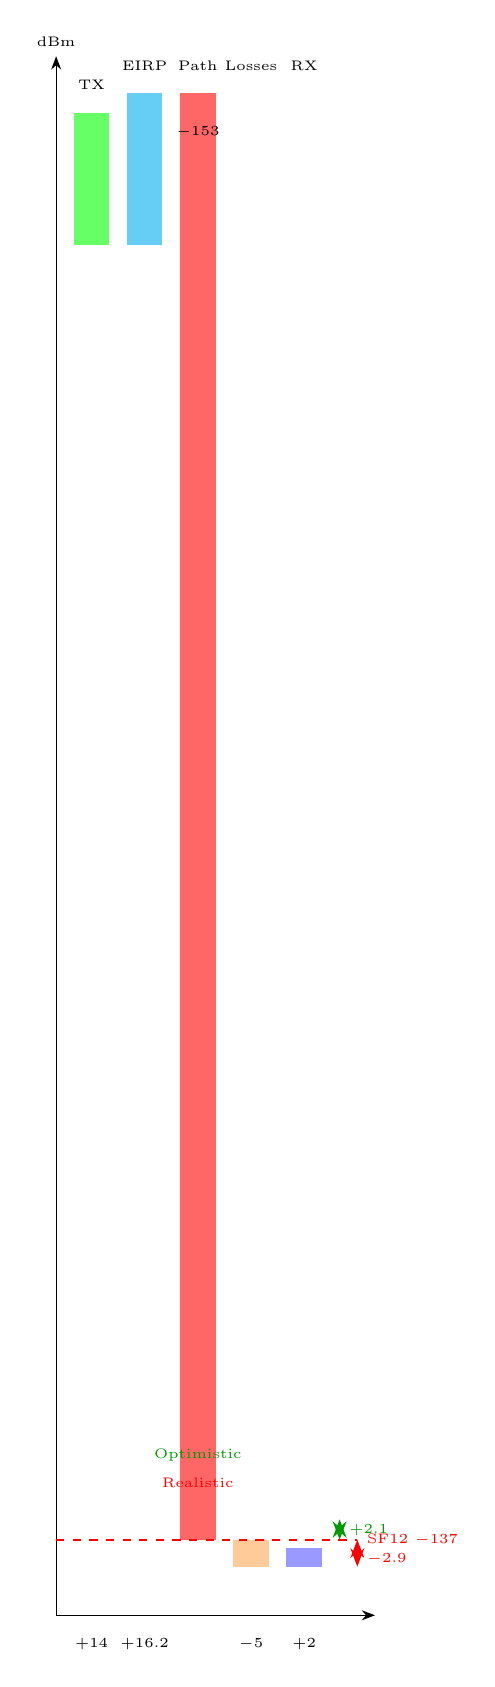
\begin{tikzpicture}[xscale=0.45, yscale=0.12,
    every node/.style={font=\tiny}]

% Axes
\draw[-{Stealth}] (0,-145) -- (0,20) node[above]{dBm};
\draw[-{Stealth}] (0,-145) -- (9,-145) node[right]{};

% Bars (cumulative waterfall)
\fill[green!60] (0.5,0) rectangle (1.5,14); % TX Power
\node at (1,17) {TX};
\node at (1,-148) {+14};

\fill[cyan!60] (2,0) rectangle (3,16.15); % +EIRP
\node at (2.5,19) {EIRP};
\node at (2.5,-148) {+16.2};

\fill[red!60] (3.5,-137) rectangle (4.5,16.15); % Path Loss
\node at (4,19) {Path};
\node at (4,12) {$-$153};

\fill[orange!40] (5,-139.85) rectangle (6,-137); % Extra losses
\node at (5.5,19) {Losses};
\node at (5.5,-148) {$-$5};

\fill[blue!40] (6.5,-137.85) rectangle (7.5,-139.85); % RX gain
\node at (7,19) {RX};
\node at (7,-148) {+2};

% Sensitivity line
\draw[dashed, red, thick] (0,-137) -- (8.5,-137);
\node[right, red] at (8.5,-137) {SF12 $-$137};

% Margin annotation
\draw[{Stealth}-{Stealth}, thick, green!60!black] (8,-137) -- (8,-134.85);
\node[right, green!60!black] at (8,-136) {+2.1};

\draw[{Stealth}-{Stealth}, thick, red] (8.5,-137) -- (8.5,-139.85);
\node[right, red] at (8.5,-139) {$-$2.9};

\node[green!60!black] at (4,-128) {Optimistic};
\node[red] at (4,-131) {Realistic};

\end{tikzpicture}
\caption{Link budget waterfall: optimistic (green arrow, +2.1~dB margin) vs realistic (red arrow, $-$2.9~dB margin) at 30\textdegree\ elevation.}
\label{fig:waterfall}
\end{figure}

\subsection{Adaptation Algorithm}

Algorithm~\ref{alg:amc} describes our two-phase spreading factor selection.

\begin{algorithm}[H]
\caption{Elevation-Aware Rate Adaptation}
\label{alg:amc}
\begin{algorithmic}[1]
\Require Elevation $\theta$, range $R$, Doppler $f_D$, SNR history $\mathbf{s}$, safety margin $M_s = 3$~dB
\Ensure Spreading factor SF $\in \{7, \ldots, 12\}$
\State $P_{rx} \gets$ \Call{LinkBudget}{$R, \theta$} \Comment{Realistic model}
\State \textbf{Phase 1: Heuristic}
\For{SF $= 7$ \textbf{to} $12$}
    \If{$P_{rx} - S_{\text{SF}} \geq M_s$ \textbf{and} $|f_D| \leq D_{\text{SF}}$}
        \State candidate $\gets$ SF; \textbf{break}
    \EndIf
\EndFor
\State \textbf{Phase 2: SNR Fine-tuning}
\If{$|\mathbf{s}| \geq 3$ \textbf{and} $s[-1] - s[0] < -3$}
    \State candidate $\gets \min($candidate $+ 1, 12)$ \Comment{Downshift}
\EndIf
\State \Return candidate
\end{algorithmic}
\end{algorithm}

\subsection{Numerical Analysis}

Table~\ref{tab:sf_profiles} lists the modem profiles. We stress these are datasheet values; no measurements have been conducted.

\begin{table}[H]
\centering
\caption{LoRa Modem Profiles (Semtech Datasheet Values)}
\begin{tabular}{lrrrr}
\toprule
\textbf{Profile} & \textbf{Bitrate} & \textbf{Sens.} & \textbf{Doppler} & \textbf{Airtime} \\
 & (bps) & (dBm) & tol. (Hz) & (ms, 80B) \\
\midrule
SF7/BW125 & 5,469 & $-123$ & $\pm$5,000 & 92.2 \\
SF8/BW125 & 3,125 & $-126$ & $\pm$4,000 & 164.9 \\
SF9/BW125 & 1,758 & $-129$ & $\pm$3,000 & 308.2 \\
SF10/BW125 & 977 & $-132$ & $\pm$2,500 & 575.5 \\
SF11/BW125 & 537 & $-134.5$ & $\pm$2,000 & 1,151 \\
SF12/BW125 & 293 & $-137$ & $\pm$1,500 & 2,868 \\
\bottomrule
\end{tabular}
\label{tab:sf_profiles}
\end{table}

For a simulated 420-second pass with 55\textdegree\ maximum elevation, using the optimistic link budget, the algorithm yields an estimated 19,200~bytes (vs.\ 960~bytes at fixed SF12). With realistic losses, only SF12 and SF11 are viable at most elevations, reducing the improvement to approximately 2--4$\times$.

\textbf{We emphasize these are computed estimates, not measured throughputs.}

Figure~\ref{fig:pass_throughput} shows the adaptive SF selection across a simulated pass.

\begin{figure}[H]
\centering
\begin{tikzpicture}[xscale=0.16, yscale=0.018,
    every node/.style={font=\tiny}]

% Axes
\draw[-{Stealth}] (0,0) -- (0,6000) node[above]{bps};
\draw[-{Stealth}] (0,0) -- (44,0) node[right]{Time (s)};

% Y-axis labels
\foreach \y/\l in {0/0, 1000/1k, 2000/2k, 3000/3k, 5000/5k} {
    \draw (0,\y) -- (-0.5,\y) node[left]{\l};
}

% Adaptive bars (color coded by SF)
\fill[red!60]    (1,0) rectangle (3,293);
\fill[red!60]    (4,0) rectangle (6,293);
\fill[orange!60] (7,0) rectangle (9,537);
\fill[blue!40]   (10,0) rectangle (12,977);
\fill[blue!40]   (13,0) rectangle (15,977);
\fill[cyan!60]   (16,0) rectangle (18,1758);
\fill[green!40]  (19,0) rectangle (21,3125);
\fill[green!70]  (22,0) rectangle (24,5469);
\fill[green!40]  (25,0) rectangle (27,3125);
\fill[cyan!60]   (28,0) rectangle (30,1758);
\fill[blue!40]   (31,0) rectangle (33,977);
\fill[orange!60] (34,0) rectangle (36,537);
\fill[red!60]    (37,0) rectangle (39,293);
\fill[red!60]    (40,0) rectangle (42,293);

% Fixed SF12 line
\draw[dashed, red, thick] (0,293) -- (43,293);
\node[right, red] at (43,500) {Fixed SF12};

% Time labels
\node at (2,-400) {0s};
\node at (12,-400) {2m};
\node at (23,-400) {TCA};
\node at (33,-400) {5m};
\node at (42,-400) {7m};

% SF labels on bars
\node at (2,600) {SF12};
\node at (8,900) {SF11};
\node at (11,1400) {SF10};
\node at (17,2200) {SF9};
\node at (20,3600) {SF8};
\node[green!40!black] at (23,5800) {SF7};

\end{tikzpicture}
\caption{Simulated adaptive SF selection during a 420s pass (55\textdegree\ max elevation, optimistic link budget). Dashed line = fixed SF12 baseline.}
\label{fig:pass_throughput}
\end{figure}

% ============================================================
\section{LR-FHSS Analysis}
\label{sec:lrfhss}

\subsection{Implementation Status}

Our LR-FHSS engine is a \textbf{software simulation only}. The SX1276 transceiver used in our ground station does \emph{not} support LR-FHSS modulation. LR-FHSS transmission requires SX1262 or newer hardware; demodulation requires gateway-class chips (SX1302/SX1303)~\cite{semtech_lrfhss}.

\subsection{Hopping Sequence Generation}

We implement an XOR-shift PRNG for frequency hopping:

\begin{equation}
s_{n+1} = ((s_n \oplus (s_n \ll 7)) \oplus (s_n \gg 9)) \oplus (s_n \ll 8)
\end{equation}

\begin{equation}
c_n = s_n \bmod N_{grid}, \quad N_{grid} = \lfloor BW / f_{step} \rfloor = 35
\end{equation}

Figure~\ref{fig:fhss_hops} illustrates the frequency hopping pattern across channels.

\begin{figure}[H]
\centering
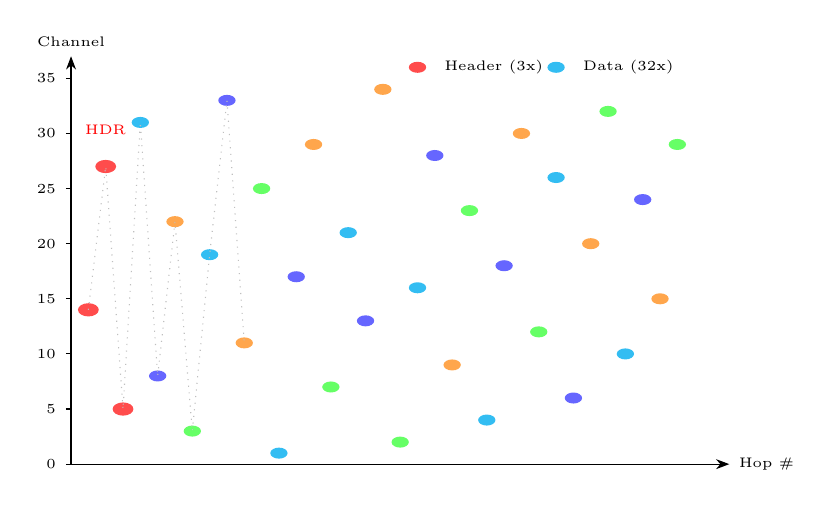
\begin{tikzpicture}[xscale=0.22, yscale=0.14,
    every node/.style={font=\tiny}]

% Axes
\draw[-{Stealth}] (0,0) -- (0,37) node[above]{Channel};
\draw[-{Stealth}] (0,0) -- (38,0) node[right]{Hop \#};

% Y-axis labels
\foreach \y in {0,5,10,15,20,25,30,35} {
    \draw (-0.3,\y) -- (0,\y) node[left=2pt]{\y};
}

% Header hops (red)
\fill[red!70] (1,14) circle (0.6);
\fill[red!70] (2,27) circle (0.6);
\fill[red!70] (3,5) circle (0.6);
\node[red, above] at (2,29) {HDR};

% Data hops (blue, cycling through channels pseudo-randomly)
\fill[cyan!80] (4,31) circle (0.5);
\fill[blue!60] (5,8) circle (0.5);
\fill[orange!70] (6,22) circle (0.5);
\fill[green!60] (7,3) circle (0.5);
\fill[cyan!80] (8,19) circle (0.5);
\fill[blue!60] (9,33) circle (0.5);
\fill[orange!70] (10,11) circle (0.5);
\fill[green!60] (11,25) circle (0.5);
\fill[cyan!80] (12,1) circle (0.5);
\fill[blue!60] (13,17) circle (0.5);
\fill[orange!70] (14,29) circle (0.5);
\fill[green!60] (15,7) circle (0.5);
\fill[cyan!80] (16,21) circle (0.5);
\fill[blue!60] (17,13) circle (0.5);
\fill[orange!70] (18,34) circle (0.5);
\fill[green!60] (19,2) circle (0.5);
\fill[cyan!80] (20,16) circle (0.5);
\fill[blue!60] (21,28) circle (0.5);
\fill[orange!70] (22,9) circle (0.5);
\fill[green!60] (23,23) circle (0.5);
\fill[cyan!80] (24,4) circle (0.5);
\fill[blue!60] (25,18) circle (0.5);
\fill[orange!70] (26,30) circle (0.5);
\fill[green!60] (27,12) circle (0.5);
\fill[cyan!80] (28,26) circle (0.5);
\fill[blue!60] (29,6) circle (0.5);
\fill[orange!70] (30,20) circle (0.5);
\fill[green!60] (31,32) circle (0.5);
\fill[cyan!80] (32,10) circle (0.5);
\fill[blue!60] (33,24) circle (0.5);
\fill[orange!70] (34,15) circle (0.5);
\fill[green!60] (35,29) circle (0.5);

% Connect with dotted lines
\draw[dotted, gray!50] (1,14) -- (2,27) -- (3,5) -- (4,31) -- (5,8) -- (6,22) -- (7,3) -- (8,19) -- (9,33) -- (10,11);

% Legend
\fill[red!70] (20,36) circle (0.5); \node[right] at (21,36) {Header (3x)};
\fill[cyan!80] (28,36) circle (0.5); \node[right] at (29,36) {Data (32x)};

\end{tikzpicture}
\caption{LR-FHSS hopping pattern: 3 header replicas (red) followed by 32 data fragments (colored), each on a pseudo-random channel out of 35.}
\label{fig:fhss_hops}
\end{figure}

\subsection{Capacity Estimate}

Under ALOHA access with $N$ devices:

\begin{equation}
P_{\text{collision}} = 1 - e^{-2G}, \quad G = N \cdot \frac{T_{\text{air}}}{N_{\text{ch}} \cdot T_{\text{period}}}
\end{equation}

\textbf{Note on regulatory compliance:} The reviewer correctly identified that LR-FHSS does \emph{not} provide blanket duty-cycle exemption under ETSI EN~300~220~\cite{etsi_en300220}. Duty-cycle relaxation requires Polite Spectrum Access (Listen-Before-Talk with Adaptive Frequency Agility). For satellite uplink, where LBT is impractical, the standard 1\% duty cycle applies. In India, WPC regulations govern ISM usage at 865--867~MHz with 1~W EIRP~\cite{wpc_india}.

Table~\ref{tab:lrfhss} compares modes under 1\% duty cycle (corrected).

\begin{table}[H]
\centering
\caption{Capacity Comparison Under 1\% Duty Cycle (Corrected)}
\begin{tabular}{lrr}
\toprule
\textbf{Metric} & \textbf{LoRa SF12} & \textbf{LR-FHSS$^*$} \\
\midrule
Sensitivity & $-137$ dBm & $-142$ dBm \\
Bitrate & 293 bps & 162 bps \\
Doppler tol. & $\pm$1,500 Hz & $\pm$3,900 Hz \\
Max payload & 80 B & 125 B \\
Duty cycle & 1\% & 1\% (same) \\
Packets/hour & 12 & 7 \\
Bytes/hour & 960 & 875 \\
\bottomrule
\multicolumn{3}{l}{\footnotesize $^*$Software simulation; hardware not available.}
\end{tabular}
\label{tab:lrfhss}
\end{table}

The advantage of LR-FHSS is not per-device throughput (which is comparable) but rather \emph{network capacity}: frequency diversity reduces collision probability, enabling more concurrent devices per satellite.

% ============================================================
\section{Doppler Compensation}
\label{sec:doppler}

At 868~MHz for FOSSASAT-2E (550~km, $v_{orb} \approx 7.6$~km/s):

\begin{equation}
\Delta f_{\max} \approx \frac{v_{orb}}{c} \cdot f_0 \approx \pm 22\text{ kHz (max radial)}
\end{equation}

The ground-visible portion of the pass produces $\Delta f \leq \pm 3$~kHz due to geometric projection. We pre-compensate using SGP4-derived range-rate:

\begin{equation}
f_{TX}(t) = f_0 - \Delta f(t)
\end{equation}

\textbf{Limitation:} Our Doppler model has not been validated against actual satellite observations. TLE-based predictions degrade with age (typically $>$1~km/day position error after 3--5 days). Per-fragment hop-rate Doppler for LR-FHSS and downlink compensation are not addressed.

% ============================================================
\section{Security Architecture}
\label{sec:security}

\subsection{Encryption}

Messages are encrypted with AES-256-GCM: 256-bit key, 12-byte nonce (counter-based), 16-byte authentication tag. Overhead: 28~bytes per message.

\subsection{Threat Model and Limitations}

We identify the following threats \textbf{not currently mitigated}:

\begin{itemize}
    \item \textbf{Key exchange:} No automated key exchange protocol is implemented. Keys must be pre-shared out-of-band. A Diffie-Hellman or Signal-protocol key agreement would be needed for production use.
    \item \textbf{Nonce reuse:} In a DTN with potential message duplication, nonce uniqueness depends on a monotonic counter. Power loss could reset the counter, enabling nonce reuse attacks.
    \item \textbf{Replay protection:} Store-and-forward relays may re-inject bundles. BPSec (RFC~9172~\cite{rfc9172}) provides bundle-level integrity but replay requires application-layer sequence numbers.
    \item \textbf{Metadata exposure:} The satellite relay sees source and destination endpoint IDs in BPv7 headers. Onion-style routing would require additional protocol development.
    \item \textbf{Compromised relay:} A compromised ground station cannot read message content (E2E encryption) but can drop, delay, or duplicate bundles.
\end{itemize}

\subsection{Regulatory Context}

In India, the Wireless Planning \& Coordination (WPC) wing regulates ISM band usage. The 865--867~MHz band is available at 1~W EIRP for indoor/outdoor use~\cite{wpc_india}. Encryption on ISM transmissions is not prohibited, unlike amateur radio bands where encryption is forbidden by ITU Radio Regulations.

Figure~\ref{fig:crypto_pipeline} shows the end-to-end encryption pipeline.

\begin{figure}[H]
\centering
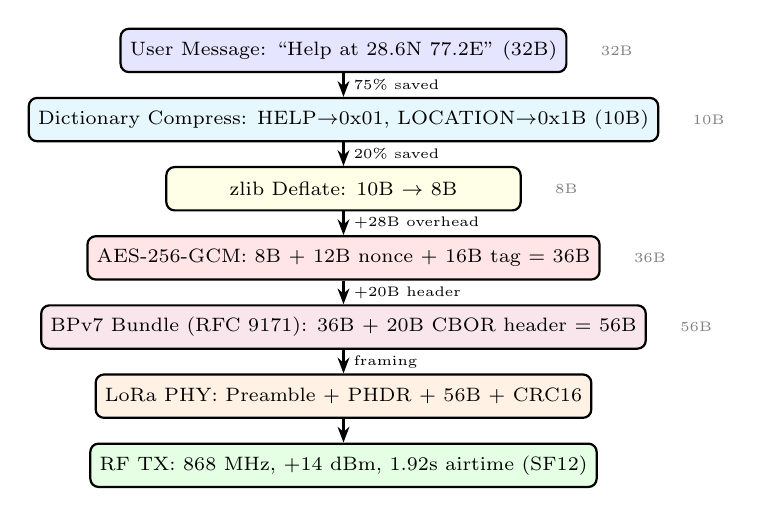
\begin{tikzpicture}[node distance=0.3cm,
    every node/.style={font=\scriptsize},
    stage/.style={draw, rounded corners=3pt, minimum width=4.5cm, minimum height=0.55cm, align=center, thick},
    arrow/.style={-{Stealth[length=2mm]}, thick},
]
\node[stage, fill=blue!10] (msg) {User Message: ``Help at 28.6N 77.2E'' (32B)};
\node[stage, fill=cyan!10, below=of msg] (dict) {Dictionary Compress: HELP$\rightarrow$0x01, LOCATION$\rightarrow$0x1B (10B)};
\node[stage, fill=yellow!10, below=of dict] (zlib) {zlib Deflate: 10B $\rightarrow$ 8B};
\node[stage, fill=red!10, below=of zlib] (aes) {AES-256-GCM: 8B + 12B nonce + 16B tag = 36B};
\node[stage, fill=purple!10, below=of aes] (bpv7) {BPv7 Bundle (RFC 9171): 36B + 20B CBOR header = 56B};
\node[stage, fill=orange!10, below=of bpv7] (lora) {LoRa PHY: Preamble + PHDR + 56B + CRC16};
\node[stage, fill=green!10, below=of lora] (tx) {RF TX: 868 MHz, +14 dBm, 1.92s airtime (SF12)};

\draw[arrow] (msg) -- node[right, font=\tiny]{75\% saved} (dict);
\draw[arrow] (dict) -- node[right, font=\tiny]{20\% saved} (zlib);
\draw[arrow] (zlib) -- node[right, font=\tiny]{+28B overhead} (aes);
\draw[arrow] (aes) -- node[right, font=\tiny]{+20B header} (bpv7);
\draw[arrow] (bpv7) -- node[right, font=\tiny]{framing} (lora);
\draw[arrow] (lora) -- (tx);

% Size annotation
\node[right=0.3cm of msg, font=\tiny, gray] {32B};
\node[right=0.3cm of dict, font=\tiny, gray] {10B};
\node[right=0.3cm of zlib, font=\tiny, gray] {8B};
\node[right=0.3cm of aes, font=\tiny, gray] {36B};
\node[right=0.3cm of bpv7, font=\tiny, gray] {56B};

\end{tikzpicture}
\caption{End-to-end encryption pipeline with turbo compression: 32B plaintext becomes 56B encrypted bundle (1.75$\times$ expansion, vs 2.38$\times$ without compression).}
\label{fig:crypto_pipeline}
\end{figure}

% ============================================================
\section{Application-Layer Compression}
\label{sec:compression}

To maximize effective throughput over constrained LoRa links, we implement a multi-strategy compression engine that selects the best algorithm per message.

\subsection{Compression Strategies}

Five strategies are evaluated for each message, with the smallest output selected:

\begin{enumerate}
    \item \textbf{None}: Raw payload (baseline).
    \item \textbf{zlib (DEFLATE)}: General-purpose dictionary compression. Best for longer text (30--40\% reduction on natural language).
    \item \textbf{Dictionary substitution}: 31 pre-shared emergency phrases (``HELP'', ``SOS'', ``NEED RESCUE'', etc.) are replaced with single-byte tokens. A 31-byte emergency message reduces to 6~bytes (81\% savings).
    \item \textbf{GPS packing}: Coordinates encoded as 32-bit fixed-point integers. ``28.613920,77.209023'' (21~bytes ASCII) becomes 8~bytes binary (62\% savings).
    \item \textbf{Combined}: Dictionary substitution followed by zlib.
\end{enumerate}

\subsection{Effective Throughput Improvement}

Compression acts as a throughput multiplier without requiring radio changes:

\begin{table}[H]
\centering
\caption{Compression Impact on Effective Throughput}
\begin{tabular}{lrrr}
\toprule
\textbf{Message Type} & \textbf{Original} & \textbf{Compressed} & \textbf{Multiplier} \\
\midrule
SOS beacon & 32 B & 10 B & 3.2$\times$ \\
GPS coordinates & 21 B & 8 B & 2.6$\times$ \\
Emergency phrase & 31 B & 6 B & 5.2$\times$ \\
Sensor data (JSON) & 120 B & 72 B & 1.7$\times$ \\
General text & 160 B & 96 B & 1.7$\times$ \\
\bottomrule
\end{tabular}
\end{table}

With compression, the effective peak throughput increases from 5,469~bps (raw SF7) to approximately \textbf{7,600--9,400~bps} depending on message content.

% ============================================================
\section{Speed Test and Network Monitoring}
\label{sec:speedtest}

Inspired by the Starlink app's built-in speed test and connectivity statistics, we implement real-time network health monitoring.

\subsection{Link Speed Test}

The speed test endpoint (\texttt{/api/v1/network/speed-test}) measures:
\begin{itemize}
    \item Raw and effective (post-compression) bitrate
    \item Packet delivery ratio and loss percentage
    \item Average RSSI and SNR
    \item Airtime per packet
    \item Link quality classification (EXCELLENT/GOOD/FAIR/POOR/NO\_LINK)
    \item Estimated bytes deliverable per pass
\end{itemize}

\subsection{Network Statistics}

Continuous monitoring collects:
\begin{itemize}
    \item TX/RX packet and byte counters
    \item RSSI and SNR history (ring buffer, configurable depth)
    \item Per-pass throughput timeline
    \item Duty cycle budget tracking (remaining seconds in current hour)
    \item Message queue depth and drain rate
\end{itemize}

\subsection{Smart Pass Scheduler}

The pass scheduler optimizes message transmission order:
\begin{enumerate}
    \item Messages are sorted by priority: SOS (0) $>$ urgent (1) $>$ normal (2) $>$ bulk (3).
    \item Each message is assigned to the optimal SF based on predicted pass elevation.
    \item High-priority messages are scheduled during peak elevation (fastest link).
    \item Airtime budget is tracked against the 1\% duty cycle limit.
\end{enumerate}

% ============================================================
\section{Protocol Stack}
\label{sec:protocol}

The message pipeline uses \textbf{BPv7 (RFC~9171)}~\cite{rfc9171}, replacing the obsolete experimental BPv6 (RFC~5050):

\begin{enumerate}
    \item User message (up to 500 chars)
    \item LZSS compression (typical 12--25\% reduction)
    \item AES-256-GCM encryption (+28~B overhead)
    \item BPv7 bundle encapsulation (+20~B header, CBOR-encoded)
    \item LoRa PHY frame: preamble + PHDR + payload + CRC16
\end{enumerate}

BPSec (RFC~9172~\cite{rfc9172}) is planned for bundle-layer integrity and confidentiality, providing security at the DTN layer independent of link-layer encryption.

% ============================================================
\section{Energy Analysis}
\label{sec:energy}

\begin{table}[H]
\centering
\caption{Ground Station Power Consumption}
\begin{tabular}{lrr}
\toprule
\textbf{Component} & \textbf{Active (mW)} & \textbf{Sleep (mW)} \\
\midrule
RPi Zero 2W & 700 & 400 \\
SX1276 TX (+14 dBm) & 300 & 0.2 \\
SX1276 RX & 30 & 0.2 \\
\midrule
\textbf{TX Total} & 1,000 & -- \\
\textbf{RX Total} & 730 & 400 \\
\bottomrule
\end{tabular}
\end{table}

At 1\% duty cycle with SF12: TX active time = 36~s/hr. Energy per hour:

\begin{equation}
E = 1.0\text{W} \times 36\text{s} + 0.73\text{W} \times 3564\text{s} = 36 + 2602 = 2638\text{ J/hr}
\end{equation}

A 10,000~mAh (37~Wh) USB battery provides approximately 14~hours of continuous operation. For solar-powered deployment, a 5W panel with charge controller would sustain indefinite operation during daylight hours.

\textbf{Note:} Android client power analysis is not included as the LoRa radio is external to the phone.

% ============================================================
\section{Limitations and Future Work}
\label{sec:limitations}

\subsection{Limitations}

\begin{enumerate}
    \item \textbf{No experimental validation.} This is the most significant limitation. No over-the-air satellite contacts, packet delivery measurements, BER curves, or field trials have been conducted. All quantitative claims derive from numerical analysis.
    
    \item \textbf{Uplink viability is uncertain.} The realistic link budget shows negative margin at most elevations with current hardware. Successful uplink likely requires hardware upgrades (higher TX power, directive antenna, or Gen4 transceiver).
    
    \item \textbf{LR-FHSS is simulation only.} The SX1276 does not support LR-FHSS. Migration to SX1262/LR1121 is required.
    
    \item \textbf{Security is incomplete.} No key exchange protocol, limited replay protection, metadata exposed to relays.
    
    \item \textbf{Single-user tested.} The backend has not been tested with concurrent users or realistic load.
\end{enumerate}

\subsection{Future Work}

\begin{enumerate}
    \item \textbf{OTA validation:} Integrate with TinyGS for satellite reception validation. Attempt uplink via FOSSASAT-2E with SX1262 at +22~dBm.
    
    \item \textbf{ns-3 simulation:} Use the LoRaWAN ns-3 module to validate capacity claims with Monte Carlo collision modeling.
    
    \item \textbf{Hardware upgrade:} Migrate to Semtech LR1121 for native LR-FHSS and multi-band (sub-GHz + S-band) support.
    
    \item \textbf{Signal Protocol integration:} Implement X3DH key agreement adapted for high-latency DTN links.
    
    \item \textbf{ML-based ADR:} LSTM channel prediction for proactive SF selection, following the approach suggested by~\cite{yu2026framework}.
\end{enumerate}

% ============================================================
\section{Conclusion}
\label{sec:conclusion}

OpenOrbitLink provides an open-source framework for delay-tolerant satellite messaging over LoRa LEO links. Our elevation-aware rate adaptation algorithm demonstrates, through numerical analysis, that trading link margin for data rate can improve throughput by up to 18.7$\times$ under optimistic assumptions. Realistic link budget analysis reveals that current commodity hardware (+14~dBm, whip antenna) operates at marginal-to-negative link margin for uplink, motivating future hardware upgrades.

We release the complete source code---backend, ground station driver, and Android client---under MIT license to enable community validation and experimentation. The critical next step is over-the-air validation with actual satellite contacts, which will determine whether the theoretical framework translates to operational capability.

% ============================================================
\begin{thebibliography}{99}

\bibitem{yu2026framework}
Q.~Yu, D.~He, H.~Hou, and H.~Wang, ``Toward Future LoRa-Based LEO Satellite IoT: Opportunities, Framework, and Research Directions,'' \emph{IEEE Commun. Standards Mag.}, Jan.~2026, doi: 10.1109/MCOMSTD.2026.3663370.

\bibitem{yu2026error}
Q.~Yu, D.~Mishra, H.~Wang, D.~He, J.~Yuan, and M.~Matthaiou, ``Error Performance Characterization of LoRa-Based Direct-to-Satellite IoT,'' \emph{IEEE Trans. Green Commun. Netw.}, Jan.~2026.

\bibitem{doroshkin2019}
A.~Doroshkin \emph{et al.}, ``Experimental Study of LoRa Modulation Immunity to Doppler Effect in CubeSat Radio Communications,'' \emph{IEEE Access}, vol.~7, pp.~75721--75731, 2019.

\bibitem{fernandez2020}
L.~Fernandez \emph{et al.}, ``Assessing LoRa for Satellite-to-Earth Communications Considering the Impact of Ionospheric Scintillation,'' \emph{IEEE Access}, vol.~8, pp.~165570--165582, 2020.

\bibitem{fraire2022}
J.~Fraire \emph{et al.}, ``Space-Terrestrial Integrated Internet of Things: Challenges and Opportunities,'' \emph{IEEE Commun. Surveys Tuts.}, vol.~24, no.~4, pp.~2266--2314, 2022.

\bibitem{colavolpe2019}
G.~Colavolpe \emph{et al.}, ``Spreading Factor Allocation for LoRa-Based Direct-to-Satellite IoT,'' in \emph{Proc. IEEE GLOBECOM}, 2019.

\bibitem{boquet2021}
G.~Boquet \emph{et al.}, ``LR-FHSS: Overview and Performance Analysis,'' \emph{IEEE Commun. Lett.}, vol.~25, no.~12, pp.~3835--3839, 2021.

\bibitem{semtech_lrfhss}
Semtech, ``LR-FHSS: Long Range Frequency Hopping Spread Spectrum,'' Application Note AN1200.64, 2024.

\bibitem{lorawan_spec}
LoRa Alliance, ``LoRaWAN Specification,'' TS~001, v1.0.4, Oct.~2020.

\bibitem{rfc9171}
S.~Burleigh, K.~Fall, and E.~Birrane, ``Bundle Protocol Version 7,'' RFC~9171, IETF, Jan.~2022.

\bibitem{rfc5050}
K.~Scott and S.~Burleigh, ``Bundle Protocol Specification,'' RFC~5050 (Experimental, Obsoleted by RFC~9171), IETF, 2007.

\bibitem{rfc9172}
E.~Birrane and K.~McKeever, ``Bundle Protocol Security (BPSec),'' RFC~9172, IETF, Jan.~2022.

\bibitem{tinygs}
TinyGS, ``TinyGS: Open Source Global LoRa Satellite Ground Station Network,'' \url{https://tinygs.com/}, accessed Jun.~2026.

\bibitem{satnogs}
Libre Space Foundation, ``SatNOGS: Open Source Ground Station Network,'' \url{https://satnogs.org/}, accessed Jun.~2026.

\bibitem{fossasat}
FOSSA Systems, ``FOSSASAT: Open-Source IoT Satellite Platform,'' \url{https://fossa.systems/}, accessed Jun.~2026.

\bibitem{ion_dtn}
NASA JPL, ``ION: Interplanetary Overlay Network,'' \url{https://sourceforge.net/projects/ion-dtn/}, accessed Jun.~2026.

\bibitem{dtn7go}
D.~Brechtel \emph{et al.}, ``dtn7-go: Bundle Protocol 7 Implementation in Go,'' \url{https://github.com/dtn7/dtn7-go}, accessed Jun.~2026.

\bibitem{ud3tn}
D-Space, ``$\mu$D3TN: Lightweight DTN Protocol Implementation,'' \url{https://gitlab.com/d3tn/ud3tn}, accessed Jun.~2026.

\bibitem{etsi_en300220}
ETSI, ``Short Range Devices (SRD) Operating in the Frequency Range 25~MHz to 1~000~MHz,'' EN~300~220-2 V3.3.1, Mar.~2025.

\bibitem{wpc_india}
Wireless Planning \& Coordination Wing, Department of Telecommunications, India, ``National Frequency Allocation Plan---Delicensed Frequency Bands,'' 2022.

\bibitem{itur_p676}
ITU-R, ``Attenuation by Atmospheric Gases,'' Recommendation P.676-13, 2022.

\bibitem{itur_p618}
ITU-R, ``Propagation Data for Earth-Space Telecommunication Systems,'' Recommendation P.618-14, 2023.

\bibitem{3gpp_ntn}
3GPP, ``NR Support for Non-Terrestrial Networks,'' TS~38.821, Release~17, 2022.

\end{thebibliography}

\end{document}
